\documentclass[10pt,a4paper]{article}
\usepackage[margin=20mm]{geometry}
\usepackage{amsmath,amssymb,booktabs,longtable,array,graphicx,hyperref,placeins}
\hypersetup{hidelinks,breaklinks=true}
\setlength{\parindent}{0pt}
\setlength{\parskip}{4pt}
\setlength{\emergencystretch}{2em}
\setlength{\LTpre}{4pt}
\setlength{\LTpost}{5pt}
\setlength{\LTcapwidth}{\textwidth}
\makeatletter
\renewcommand\section{\@startsection{section}{1}{\z@}%
  {-2ex \@plus -.5ex \@minus -.2ex}{.8ex \@plus .2ex}%
  {\normalfont\large\bfseries}}
\renewcommand\paragraph{\@startsection{paragraph}{4}{\z@}%
  {1ex \@plus .2ex \@minus .1ex}{-1em}%
  {\normalfont\normalsize\bfseries}}
\renewcommand*\l@section{\@dottedtocline{1}{0em}{2.5em}}
\makeatother
\renewcommand{\thesection}{S\arabic{section}}
\renewcommand{\thetable}{S\arabic{table}}
\renewcommand{\thefigure}{S\arabic{figure}}
\title{Online Supplement to Hard to Beat: Historical Rules versus Conditional Quantile Models for Peak Net-Position Limits}
\author{}
\date{}
% Cached Latin Modern OpenType faces; no font download or system install.
% Scalable Computer Modern-derived faces avoid absent optical-size TFM files.
\usepackage[TU]{fontenc}
\DeclareFontFamily{TU}{qflmr}{}
\DeclareFontShape{TU}{qflmr}{m}{n}{<->\UnicodeFontFile{lmroman10-regular}{\UnicodeFontTeXLigatures}}{}
\DeclareFontShape{TU}{qflmr}{m}{it}{<->\UnicodeFontFile{lmroman10-italic}{\UnicodeFontTeXLigatures}}{}
\DeclareFontShape{TU}{qflmr}{m}{sl}{<->ssub*qflmr/m/it}{}
\DeclareFontShape{TU}{qflmr}{m}{sc}{<->ssub*qflmr/m/n}{}
\DeclareFontShape{TU}{qflmr}{bx}{n}{<->\UnicodeFontFile{lmroman10-bold}{\UnicodeFontTeXLigatures}}{}
\DeclareFontShape{TU}{qflmr}{bx}{it}{<->\UnicodeFontFile{lmroman10-italic}{\UnicodeFontTeXLigatures embolden=1.8;}}{}
\DeclareFontShape{TU}{qflmr}{b}{n}{<->ssub*qflmr/bx/n}{}
\DeclareFontShape{TU}{qflmr}{b}{it}{<->ssub*qflmr/bx/it}{}
\DeclareFontFamily{TU}{qflmtt}{}
\DeclareFontShape{TU}{qflmtt}{m}{n}{<->\UnicodeFontFile{lmmono10-regular}{}}{}
\DeclareFontShape{TU}{qflmtt}{m}{it}{<->ssub*qflmtt/m/n}{}
\DeclareFontShape{TU}{qflmtt}{bx}{n}{<->ssub*qflmtt/m/n}{}
\renewcommand{\rmdefault}{qflmr}\renewcommand{\ttdefault}{qflmtt}
\normalfont

\begin{document}
\maketitle
This supplement contains proofs, reproducible method definitions, source summaries and every saved decision. The complete preceding supplement, including all cell tables, failed numerical attempts and counterexamples, is preserved in \href{https://github.com/ByronLi0207/financial-mathematics-paper-20261020/blob/submission-final/EXTENDED_RESULTS.md}{EXTENDED RESULTS}. No financial analysis or saved result is changed by this shorter presentation.
\setcounter{tocdepth}{1}
\tableofcontents
\medskip
\section{Peak properties and their proofs}\label{sup:floor}\label{sup:levy}

We forecast the sampled maximum of the absolute position, including
the observed issue position. Write \(B=|N_t|\) and let \(Y\ge B\) almost surely,
with \(B\) measurable at the forecast origin. For \(0<\tau<1\), the pinball score is
\(\rho_\tau(u)=\tau u_+ +(1-\tau)(-u)_+\). A lower inverse conditional quantile
is \(q_\tau=\inf\{c:F(c\mid\mathcal F_t)\ge\tau\}\).

\paragraph{Proposition 1: floor projection.}
Replacing a report \(c\) by \(\max(B,c)\) weakly reduces its score at every possible
outcome. At the population conditional quantile, the strict breach probability
is at most \(1-\tau\). These are distinct statements: projection applies to any
report; the tail qualification requires the true conditional quantile.
Here \(q=q_\tau\), and \(\alpha\) denotes the stated nominal tail bound.
\[
\rho_\tau(Y-c)-\rho_\tau(Y-\max\{B,c\})=\tau(B-c)_+,\qquad \Pr(Y>q\mid\mathcal F_t)\le\alpha.
\]
\paragraph{Proof.}
If \(c\ge B\), the replacement changes nothing. If \(c<B\), both errors
\(Y-c\) and \(Y-B\) are nonnegative, so their score difference is
\(\tau(B-c)\). This proves the pointwise identity without a density assumption.
Right continuity of the conditional distribution gives
\(F(q_\tau\mid\mathcal F_t)\ge\tau\), hence
\(\Pr(Y>q_\tau\mid\mathcal F_t)\le1-\tau\). An atom at the quantile can make
this strict; exact nominal hit frequency is not required for a valid upper
quantile. A fitted report does not automatically inherit this population claim.
\hfill\textit{QED}

\paragraph{Why the floor matters.}
The sampled maximum equals the current magnitude whenever the recorded future
path remains inside its current absolute-position band. This can create an atom
even when later signed observations are continuous. The existence of a floor
alone does not imply an atom: an outcome uniformly distributed above the floor
provides a counterexample. Equality-based coverage tests therefore diagnose
their stated equalities, rather than every possible valid upper-quantile report.

\paragraph{Endpoint marginals do not identify the peak.}
The exact artificial constructions in \href{https://github.com/ByronLi0207/financial-mathematics-paper-20261020/blob/revision-v7-final/notes/revision-v5-novelty/theory-source.json}{the formal example record}
hold each future-time marginal fixed while changing temporal dependence.
Comonotone and disjoint rare events then give different peak quantiles.
The example is a logical construction, not another financial dataset or an
estimated mechanism. Forecast evaluation must use the ordered path response
and the information available at its actual origin.

\paragraph{Takeaway.}
Known-floor projection is an elementary pointwise improvement. It does not
establish empirical calibration, identify the conditional distribution, or turn
a fitted endpoint forecast into a forecast of a path maximum.

\paragraph{Proposition 2: the classical endpoint bound.}
Let future real increments \(X_1,\ldots,X_H\) be independent and individually
symmetric about zero. Set \(S_0=0\), \(S_h=\sum_{j=1}^hX_j\), and fix a starting
position \(x\), with absolute magnitude \(B\). Equal increment laws and finite moments are unnecessary.
For the population absolute-displacement quantile at level \(1-\alpha/2\),
\(q=\inf\{c:\Pr(|S_H|\le c)\ge1-\alpha/2\}\), the classical scalar maximal
inequality and the triangle inequality give
\[
\Pr\!\left(\max_{0\le h\le H}|x+S_h|>B+q\right)\le\Pr\!\left(\max_h|S_h|>q\right)\le2\Pr(|S_H|>q)\le\alpha.
\]
This is a direct application of the classical L\'evy inequality, not a new
maximal inequality.

\paragraph{Proof, including strict events and atoms.}
For \(c\ge0\), let \(\eta\) be the first index with \(|S_\eta|>c\). On
\(\{\eta=k,S_k>c\}\), the remaining sum \(R_k=S_H-S_k\) is independent of
the information through \(k\) and is symmetric. Therefore \(\Pr(R_k\ge0)\ge1/2\),
including a possible atom at zero, and that weak sign keeps \(S_H>c\).
On the corresponding negative crossing, \(R_k\le0\) keeps \(S_H<-c\), also
with probability at least one half. Summing over the disjoint crossing events
gives \(\Pr(\max_h|S_h|>c)\le2\Pr(|S_H|>c)\). The argument covers \(c=0\).
Finally, \(\max_{0\le h\le H}|x+S_h|\le |x|+\max_h|S_h|\), and right
continuity gives the required strict tail bound at \(q\). \hfill\textit{QED}

\paragraph{Conditional use and empirical implementation.}
For an observed random anchor, the same argument must hold under its
forecast-origin conditional law, with the corresponding conditional population
endpoint quantile. Conditional independence and symmetry about zero cannot be inferred from unconditional marginals. The empirical endpoint plug-in adds the current
floor to a historical absolute-displacement order statistic. Overlapping labels,
estimated quantiles and changing dependent histories provide no automatic
inheritance of this population bound or a pinball-risk ordering.

\paragraph{Two different failure mechanisms.}
Dependence can destroy the inequality: take \(X_1=Z\), \(X_2=-Z\), with
\(Z\in\{-1,1\}\) equally likely. The endpoint is zero, while the sampled
maximum is one. Separately, replacing the required absolute-displacement
quantile by a generic one-sided endpoint quantile can fail even for independent
symmetric increments. The exact finite example is preserved in the formal
example record. These logical counterexamples are separate from the Gaussian
Monte Carlo cases below; a nonviolating simulation does not prove a theorem
extension.

\paragraph{Takeaway.}
The bound supplies a clear population benchmark under explicit assumptions;
the empirical report remains a model to validate, not a coverage certificate.

\FloatBarrier


\section{Forecast construction and comparison methods}\label{sup:ar}\label{sup:rank}\label{sup:wp2}\label{sup:wp3}\label{sup:coherence}\label{sup:implementation}

\paragraph{Completed labels and update clocks.}
At a scheduled refit \(\kappa\), the latest mature peak response origin is
\(\kappa-H\). A history of \(W\) mature peak responses therefore uses
\(\{\kappa-H-W+1,\ldots,\kappa-H\}\), with every target ending by that refit.
Training transforms, scales, coefficients and historical pools are held until
the next scheduled refit. The current observed position may still change at
each forecast issue. Replacing that issue anchor by the refit anchor changes
the forecasting procedure.

\paragraph{Regression and local quantiles.}
The regression objective uses a training-normalized headroom response, an
unpenalized intercept and a ridge penalty on slopes. Projection is applied when
issuing the report and evaluating its validation score, not inside the fitted
training objective. Local methods use training-only standardized predictors,
fixed neighbour menus and duplicate-preserving order statistics. A selected
whole-pool local quantile is an exact historical identity, not a failed-fit
fallback. Scale-adjusted neighbours change responses as well as retrieval.

\paragraph{Numerical eligibility.}
The accepted solver records primal and dual residuals, objectives, feasibility and the gap between the primal and dual objectives. Ill-conditioned, nonfinite, unsupported-rank and failed candidate
states retain their original statuses under each named selection contract.
A mandatory-candidate failure blocks a procedure when its contract requires
every candidate. The original full regression has that requirement; the
four-feature selector may choose among completed eligible candidates. A failed
selected evaluation never receives a replacement penalty or a shortened score.
Changing the ridge menu changes the procedure even when feature definitions
stay fixed. A numerical certificate does not establish financial accuracy,
economic relevance, inferential validity or production continuity.
No production continuity or fallback policy is evaluated here.

\paragraph{Working-reference inference.}
Saved unconditional loss differences use the recorded Bartlett-HAC convention;
HLN and doubled-bandwidth sensitivities are labeled separately. Separate
families and later reporting partitions do not erase the wider selection
history. Coverage references distinguish full-grid Kupiec from the
transition-conditional Christoffersen joint likelihood, which conditions on
the initial hit. Small sparse grids and boundary likelihoods retain their
original status. Neither a nonrejection nor a small working-reference p value
proves conditional coverage or supplies selection-adjusted confirmation.

\paragraph{Common-pool construction distances.}
On one nonempty historical episode set, compare the historical headroom,
translated-path and historical-peak reports using the same available order
statistic. Each episode peak includes its starting observation. A translated
path changes each level by the same anchor difference, so its absolute peak
changes by at most that difference. Flooring is nonexpansive and commutes with
the fixed order statistic. The headroom construction has the corresponding
bound in the difference of anchor magnitudes. Thus
\[
|C^{\rm headroom}-C^{\rm peak}|\le\max_i\bigl||N_i|-B\bigr|,\qquad
|C^{\rm translated}-C^{\rm peak}|\le\max_i|N_i-x|.
\]
For a proof of the order-statistic step, paired coordinatewise differences
bounded by a radius imply that each empirical quantile lies below the other
plus that radius; reverse the roles for the second inequality. These
deterministic same-pool bounds do not order financial accuracy or coverage.
Changing historical rows on one side invalidates the common-pool argument.

Exact menus, numerical tolerances, failures and diagnostic tables remain in
\href{https://github.com/ByronLi0207/financial-mathematics-paper-20261020/blob/revision-v7-final/EXTENDED_RESULTS.md}{EXTENDED RESULTS} and the dated source records.

The ordinary empirical quantile and the corrected empirical rule use
the same completed pool, refit times and issue floor. The former takes the
lower empirical pinball minimizer; the latter uses the specified add-one rank.
When the product of the probability level and pool size is an integer, adjacent reports can be the two endpoints of the same empirical minimizer interval. Calling the lower report a
uniquely optimal comparator would therefore be wrong. At the short weekly pool,
the noninteger rank distinction differs.
The full rank comparison is retained in \href{https://github.com/ByronLi0207/financial-mathematics-paper-20261020/blob/submission-final/EXTENDED_RESULTS.md#asmbi-extended-s08}{complete earlier results}.

At each original refit, estimate an intercept-bearing level recursion
using each unique mature adjacent transition once. Replaying a historical ordered
residual block from the current position gives the exact algebraic identity
\[
M_{i,h}(x)=N_{i+h}+\widehat\phi^{\,h}(x-N_i),\qquad M_{i,0}(x)=x.
\]
The empirical peak uses the same completed scenario origins, response rank,
floor and refit schedule as its matched historical controls. Finite negative or
above-unit coefficients were eligible, not clipped; all observed fitted
coefficients in the saved run happened to lie inside the unit interval.
Their descriptive means are not identified data-generating parameters.
The \href{https://github.com/ByronLi0207/financial-mathematics-paper-20261020/blob/submission-final/EXTENDED_RESULTS.md#asmbi-extended-s07}{extended residual-replay results} retain the complete comparisons.

The finite delayed ACI-style wrapper adapts to past strict hits after their entire peak labels mature. Its score pool contains only completed residual
scores and uses the specified finite memory. The base-plus-score quantile is
projected onto the known floor. The adaptive alpha state is projected to the
current feasible range; the rank-zero convention issues the floor. Gamma was
selected by coverage distance, then pinball loss and the fixed tie rule, a
coverage-first selection criterion distinct from original regression fitting.
No canonical ACI theorem is imported to this modified procedure.

The headroom SAV method adapts a CAViaR recursion, rather than replicating a
return-VaR model. The completed headroom response is normalized by its
training-only scale; the recursive report is multiplied back by that same
scale and then floor-projected. Its fixed bounded optimizer and starts retain
all eligibility and convergence failures; a complete fit is not a proof of a
global optimum. Selection state carries across the unissued chronological gap.

The median combination lowers Treasury-bill loss by 4.0\%, while the mean combination raises it by 2.8\%.

Fixed report combinations use the matched historical and original
regression reports at identical origins. Their arithmetic mean is untuned.
The median also requires the original selected plain local-quantile report;
neither a smaller predictor model nor the endpoint plug-in substitutes for
that missing constituent. Combining floor-respecting reports preserves the floor, but does not guarantee a conditional quantile or a score below that of the best constituent. Identical reports generate an NA equal-loss p value rather
than a manufactured significance result.

Realized peaks are ordered as the forecast horizon grows, but
independently fitted reports use horizon-specific mature peak responses and can
cross. The extended crossing comparisons keep all common forecast times.
Repairing a long-horizon report upward can worsen pinball loss; target ordering
alone does not identify a universally beneficial repair.
The \href{https://github.com/ByronLi0207/financial-mathematics-paper-20261020/blob/submission-final/EXTENDED_RESULTS.md#asmbi-extended-s22}{extended crossing results} retain the complete comparisons.

\FloatBarrier


\section{Sources, chronological samples and reporting dates}\label{sup:v10-cftc}

The source units and chronological samples are retained below. Monetary summaries and complete within-series statistics remain in Main Table 2; contract counts are not pooled with currency exposures.
\begin{table}[htbp]\centering
\caption{Sources, sample sizes and existing chronological splits.}\label{tab:supplement-data}
\begingroup\fontsize{7.5}{9}\selectfont\setlength{\tabcolsep}{2pt}
\textit{Panel A. Sources, aligned samples and existing split dates}\\[3pt]
\begin{tabular}{@{}lllllll@{}}
\toprule
Data & Frequency & Series / records & Unit & Sample & Validation & Evaluation \\
\midrule
FX, hourly & Hourly & 1 / 18,576 & USD mn & 2014-02 to 2017-01 & 2015-10 to 2015-12 & 2016-01 to 2017-01 \\
FX, daily & Day end & 1 / 930 & USD mn & 2014-02 to 2017-01 & 2015-02 to 2015-04 & 2015-05 to 2016-12 \\
Treasury bills & Weekly & 1 / 706 & USD mn & 2013-04 to 2026-10 & 2019-07 to 2020-07 & 2021-01 to 2026-04 \\
NY Fed panel & Weekly & 12 / 706 & USD mn & 2013-04 to 2026-10 & 2019-07 to 2020-07 & 2021-01 to 2026-04 \\
CFTC panel & Weekly & 17 / 877 & Contracts & 2010-01 to 2026-10 & 2020-08 to 2021-08 & 2021-09 to 2026-09 \\
\bottomrule
\end{tabular}
\endgroup\end{table}

The source is the CFTC TFF futures-only historical backcast for 2006--2016 plus annual 2017--2026 files. The retained observations begin in 2010. All eleven original source records remain public; no other new financial data were acquired.

A complete generated calendar contains 877 Monday-labeled report weeks, from 2010-01-04 through 2026-10-19. Economic position dates are retained separately. A code needs one valid observation per week, a stable exchange and stable contract units. Missing weeks, duplicates and changes disqualify a contract rather than trigger interpolation or splicing. Known consolidation prefixes 13874,20974,12460 are excluded before ranking. This conservative rule is broader than the documented plus-suffixed codes. Full-period mean open interest ranks survivors, with literal-code ties. Seventeen of 141 observed codes qualify; the top-twenty cap never changes that count.
The \href{https://github.com/ByronLi0207/financial-mathematics-paper-20261020/blob/revision-v10b/results/v10/cftc/eligibility.json}{complete code-level eligibility and exclusions} preserve every screening decision.

Validation indices are 553--604; evaluation indices are 611--870. All labels use horizon six, leaving six unissued origins between the segments. Validation position dates are 2020-08-11--2021-08-03; the last validation label ends 2021-09-14. Evaluation position dates are 2021-09-21--2026-09-08; the last evaluation label ends 2026-10-20. Training labels at refit r span r-H-W+1 through r-H. Monday labels index the inherited feature calendar; they do not claim Monday public availability. Actual positions are normally measured Tuesday and released Friday at 15:30 Eastern. Holiday, shutdown and ION-related publication delays prevent a first-release interpretation.

The selected category series are listed below. Net positions equal dealer long minus short in raw contract counts. Equal-weight median percentage changes preserve within-contract units; they are not common-dollar portfolio risk.
\begin{center}\scriptsize\begin{longtable}{lp{7.1cm}rr}
\caption{Eligible CFTC contracts and unchanged recorded open-interest summaries.}\label{tab:cftc-source-inventory}\\
\toprule Code & Latest contract name & Mean open interest & Weeks \\\midrule\endfirsthead
\toprule Code & Latest contract name & Mean open interest & Weeks \\\midrule\endhead
044601 & UST 5Y NOTE - CHICAGO BOARD OF TRADE & 3479174.2 & 877 \\
043602 & UST 10Y NOTE - CHICAGO BOARD OF TRADE & 3344673.4 & 877 \\
042601 & UST 2Y NOTE - CHICAGO BOARD OF TRADE & 2170647.9 & 877 \\
045601 & FED FUNDS - CHICAGO BOARD OF TRADE & 1282757.7 & 877 \\
020601 & UST BOND - CHICAGO BOARD OF TRADE & 999944.0 & 877 \\
099741 & EURO FX - CHICAGO MERCANTILE EXCHANGE & 503616.5 & 877 \\
1170E1 & VIX FUTURES - CBOE FUTURES EXCHANGE & 356897.7 & 877 \\
097741 & JAPANESE YEN - CHICAGO MERCANTILE EXCHANGE & 210863.1 & 877 \\
096742 & BRITISH POUND - CHICAGO MERCANTILE EXCHANGE & 197853.5 & 877 \\
095741 & MEXICAN PESO - CHICAGO MERCANTILE EXCHANGE & 174995.0 & 877 \\
090741 & CANADIAN DOLLAR - CHICAGO MERCANTILE EXCHANGE & 166229.3 & 877 \\
232741 & AUSTRALIAN DOLLAR - CHICAGO MERCANTILE EXCHANGE & 154802.4 & 877 \\
33874A & E-MINI S\&P 400 STOCK INDEX - CHICAGO MERCANTILE EXCHANGE & 75156.1 & 877 \\
240743 & NIKKEI STOCK AVERAGE YEN DENOM - CHICAGO MERCANTILE EXCHANGE & 59766.6 & 877 \\
092741 & SWISS FRANC - CHICAGO MERCANTILE EXCHANGE & 57197.3 & 877 \\
098662 & USD INDEX - ICE FUTURES U.S. & 52473.9 & 877 \\
112741 & NZ DOLLAR - CHICAGO MERCANTILE EXCHANGE & 44292.0 & 877 \\
\bottomrule\end{longtable}\end{center}

The six methods are corrected-rank F, ordinary I, four- and thirty-three-predictor regression, and finite delayed calibration of historical headroom and full regression. Both regressions use the six-point menu. The paired ACI wrappers retain the existing finite calibration with delayed matured feedback; no asymptotic coverage claim is attached. The complete 204 method cells finish without a numerical retry. The full cell CSV and trace ZIP retain absolute scores, breaches, selected penalties and gamma values.

For the CFTC delayed wrappers, gamma belongs to $\{.001,.005,.01,.05\}$. Completed candidates rank by validation coverage-distance, then pinball loss, then smaller gamma. Initialization requires at least nineteen matured scores. Updates wait for the full six-record label, and evaluation carries the validation state. The six unissued gap origins create no artificial reports or feedback events. These settings accompany histories 52/260, 52 validation origins, 260 evaluation origins and 13-record refits; none is retuned after evaluation.

The complete ingestion chronology, exclusions and original failed preparation records remain in \href{https://github.com/ByronLi0207/financial-mathematics-paper-20261020/blob/submission-final/EXTENDED_RESULTS.md#asmbi-extended-s30}{complete earlier results}.

\FloatBarrier


\section{Fixed simulation designs and retained failures}\label{sup:simulation-original}\label{sup:simulation-primary}\label{sup:simulation-secondary}\label{sup:v8-mc}\label{sup:v9-legacy-mc}\label{sup:v9-stability}\label{sup:v10-menu}

The simulation compares inherited reports for mean-reverting position levels,
not positively autocorrelated increments and not a fitted reproduction of either
financial source. It uses
\[
N_t=\phi N_{t-1}+\varepsilon_t,\qquad
\varepsilon_t=\sqrt{v_t}z_t,\qquad
v_t=\omega+a\varepsilon_{t-1}^{2}+bv_{t-1},\qquad
z_t\stackrel{\mathrm{iid}}{\sim}\mathcal N(0,1).
\]
The level persistences are \(\phi\in\{0.7,0.9,0.98\}\), variance persistences
\(p=a+b\in\{0,0.9,0.98\}\), histories \(W\in\{52,260,720,2880\}\), and horizons
\(H\in\{6,24\}\). For the increasing variance-persistence settings, the
\((\omega,a,b)\) triples are \((1,0,0)\), \((0.1,0.05,0.85)\), \((0.02,0.05,0.93)\). Each innovation has unit unconditional
variance under the specified recursion. Initial level and variance are fixed;
a burn-in of 20000 observations precedes 3264 retained observations.
This is a long-burn approximation, not an exact stationary initialization.
The common hourly calendar has no simulated calendar effect.

There are 32 independent repetition streams, with master entropy 2026102408 and
common normal innovations across conditions within a repetition. Validation
uses origins 3072--3143; evaluation uses 3168--3239, with
72 overlapping issues and a refit every 24 records. Repetition, not
issue or grid cell, is the Monte Carlo uncertainty unit. Training uses exactly
\(W\) origins \(r-H-W+1,\ldots,r-H\), with every label ending by refit \(r\).
The current-position floor and query features use the actual issue state.
The full model keeps its original predictors and the four-feature model its
original four; their penalty menus and failure rules differ, so their contrast
is not an isolated intervention on predictor count.

For each cell, let \(A_j\) and \(B_j\) be regression and matched-historical mean losses in repetition \(j\), and \(R\) the planned number of repetitions. The
reported relative change and its delta-method Monte Carlo standard error are
\[
\widehat\Delta=100\left(\dfrac{\overline A}{\overline B}-1\right),\qquad
\operatorname{MCSE}(\widehat\Delta)=
\dfrac{100\,s(A_j-\widehat rB_j)}{\sqrt R\,\overline B},\qquad
\widehat r=\dfrac{\overline A}{\overline B}.
\]
Sample standard deviations use divisor \(R-1\). Breach-rate errors use the
between-repetition standard deviation divided by
\(\sqrt R\). Strict wins require \(A_j<B_j\), with error
\(\sqrt{\widehat\pi(1-\widehat\pi)/R}\). At zero or all wins that plug-in error is
zero without implying certainty; the worst-case error bound is
\(0.5/\sqrt R\), or 8.84 percentage points here. The short evaluation segments,
common innovations across cells, and fixed process family limit a regime claim.

The fixed descriptive clear-gain screen requires all 32 paired repetitions,
\(\widehat\Delta+2\operatorname{MCSE}(\widehat\Delta)<0\), and a strict-win fraction of at least \(0.75\). Its target is \(H=6\), \(W\ge 720\),
\(p\ge 0.9\). Support additionally requires at least 6 of 12
clear-gain target cells and none among the 60 outside cells. Each regression
has only 2 target gains and 6 outside gains. The recorded conclusion
is \textbf{MISMATCH}: both the target count and the no-outside requirement fail.
This screen has no family-wide significance guarantee and supplies no new
population endpoint-bound guarantee under dependent financial paths.

\begingroup
\renewcommand{\footnotesize}{\fontsize{9}{10.5}\selectfont}
The complete two-regression 72-cell tables remain unchanged in \href{https://github.com/ByronLi0207/financial-mathematics-paper-20261020/blob/0d2526cc69092c5158437a0509613bac5e86d47f/submission-jof/supplement.pdf}{v9 Tables S26--S27} and their native fields in the saved controlled simulation. All adverse, failed and unavailable statuses retain their original meanings. The preceding design and prediction outcomes refer to that entire grid, not a successful subset.
\endgroup

One declared candidate failed its numerical criterion; the fixed completed-candidate selector retained that failure and selected an eligible completed alternative. The original full-regression selector requires every declared candidate. \href{https://github.com/ByronLi0207/financial-mathematics-paper-20261020/blob/submission-final/EXTENDED_RESULTS.md#asmbi-extended-s24}{All candidate and procedure statuses} retain the complete numerical details.

These are the existing fixed-seed Gaussian experiments, not newly run
simulations or calibrated replicas of either financial source. Every reported
rate is a probability, not a percentage. The peak includes the initial level;
the endpoint event concerns absolute displacement from that initial level.
Each path cell has 100000 paths.
L/Stat starts the level AR in stationarity; L/Abs fixes its absolute-level
tail anchor; L/Sig is the separate signed-level tail-anchor sensitivity.
I/Zero accumulates stationary AR increments from a zero position.
M denotes a stationary-marginal endpoint threshold; C denotes a distinct
fixed-start conditional endpoint oracle. Threshold partners sharing a seed use
the same paths, not independent repetitions.
The original tables in the extended results retain the original increment, corrected primary and secondary simulation results.

The corrected level process is
\(N_h=\phi N_{h-1}+\varepsilon_h\), with independent Gaussian innovations
of variance \(1-\phi^2\) and unit stationary level variance. Its stationary
increments have lag correlation
\(\rho_X(k)=-(1-\phi)\phi^{k-1}/2\), so this mechanism differs from a
positively persistent increment AR. The fitted financial coefficient describes
levels, making the level equation the relevant illustrative mechanism.
The negative-increment family is a separate sensitivity, with stationary
increments and nonstationary cumulative levels.

For stationary random starts, absolute endpoint displacement has
variance \(2(1-\phi^H)\). At a fixed start \(x\), its conditional Gaussian
mean and variance are \((\phi^H-1)x\) and \(1-\phi^{2H}\). Thus holding the
stationary-marginal endpoint threshold across starts does not condition on a
large anchor. The conditional-oracle sensitivities in the extended results are distinct thresholds
on shared paths; neither is an oracle for the maximum.

\subsection{Isolating the penalty menu}\label{sec:extensions}

The weekly failures motivate a closer look at the penalty menu in calibrated simulations. Earlier stationary comparisons already produce large short-history regression losses. The fitted constant and switching arms use thirteen pre-evaluation weekly calibrations. The earlier stability screen rejects seven series pointwise and two after Holm correction. The extended results retain the earlier calibrated simulations and stability diagnostics.

The paired menu experiment changes only the ridge candidate menu and the stated exact-tie rule. It adds penalties one, ten and the intercept-only limit to full regression. Both regressions use the six-point menu. All paths, innovations, source calibrations and forecasting clocks match the earlier experiment. Thirty-two paired repetitions contribute to each complete source median. This isolates the executed menu comparison within these calibrated laws. The expanded procedure can choose ordinary I. Stronger finite penalties and access to I are not separately identified; near-parity loss alone supplies no evidence of added feature value.

The expanded full-regression medians move close to historical headroom in both arms (Table~\ref{tab:v10-menu-isolation}). Figure~\ref{fig:mechanism} displays these across-source medians and their descriptive spread. Both arms improve in every source. The constant-arm near-parity prediction and the paired-improvement prediction hold. The switching-minus-constant difference misses the pre-specified five-percentage-point increase. This outcome supports the menu explanation for these simulated losses; it leaves the empirical frequency mechanism unresolved.

\begin{table}[t]\centering\footnotesize
\setlength{\tabcolsep}{2pt}
\caption{Penalty-menu isolation on matched calibrated paths. Entries are the median relative loss (\%) across all 13 source medians, with the descriptive source IQR in brackets.}
\label{tab:v10-menu-isolation}
\begin{tabular}{lllrrr}\toprule
Arm & History & Regression & Original menu & Expanded menu & Missing sources \\
 & & & Median [IQR] & Median [IQR] & Original / expanded \\ \midrule
Constant & 52 & Full regression & \makebox[3.0em][r]{116.24} [\makebox[3.1em][r]{92.90}, \makebox[3.2em][r]{124.34}] & \makebox[3.0em][r]{0.21} [\makebox[3.1em][r]{-0.52}, \makebox[3.2em][r]{0.98}] & 0 / 0 \\
Constant & 52 & Four-feature & \makebox[3.0em][r]{-0.02} [\makebox[3.1em][r]{-1.55}, \makebox[3.2em][r]{1.73}] & \makebox[3.0em][r]{0.44} [\makebox[3.1em][r]{-1.69}, \makebox[3.2em][r]{1.90}] & 0 / 0 \\
Constant & 260 & Full regression & \textsc{NA} & \textsc{NA} & 1 / 1 \\
Constant & 260 & Four-feature & \makebox[3.0em][r]{-1.21} [\makebox[3.1em][r]{-1.69}, \makebox[3.2em][r]{-0.54}] & \makebox[3.0em][r]{-1.13} [\makebox[3.1em][r]{-1.69}, \makebox[3.2em][r]{-0.64}] & 0 / 0 \\
Switching & 52 & Full regression & \makebox[3.0em][r]{121.40} [\makebox[3.1em][r]{101.92}, \makebox[3.2em][r]{131.26}] & \makebox[3.0em][r]{-0.23} [\makebox[3.1em][r]{-1.88}, \makebox[3.2em][r]{0.98}] & 0 / 0 \\
Switching & 52 & Four-feature & \makebox[3.0em][r]{-0.03} [\makebox[3.1em][r]{-2.03}, \makebox[3.2em][r]{3.22}] & \makebox[3.0em][r]{0.38} [\makebox[3.1em][r]{-2.17}, \makebox[3.2em][r]{3.17}] & 0 / 0 \\
Switching & 260 & Full regression & \textsc{NA} & \textsc{NA} & 1 / 1 \\
Switching & 260 & Four-feature & \makebox[3.0em][r]{-0.27} [\makebox[3.1em][r]{-0.66}, \makebox[3.2em][r]{0.23}] & \makebox[3.0em][r]{-0.28} [\makebox[3.1em][r]{-0.75}, \makebox[3.2em][r]{0.48}] & 0 / 0 \\
\bottomrule\end{tabular}
\par\vspace{2pt}\begin{minipage}{.98\linewidth}\footnotesize
Each source median uses all 32 matched repetitions with relative loss $100(\overline L_{QR}/\overline L_F-1)$; positive values mean higher regression loss, and NA retains unavailable all-source summaries without substituting successful subsets.
Displays are rounded, while pre-specified decisions use saved full-precision operands; the two regression variants retain their stated predictor sets.
The expanded four-feature exact-tie rule prefers stronger penalties, unlike its original rule; saved exact ties: 0, changed selections: 0.
\end{minipage}\end{table}




\href{https://github.com/ByronLi0207/financial-mathematics-paper-20261020/blob/submission-final/EXTENDED_RESULTS.md#asmbi-extended-s27}{The legacy calibrated simulation and every failed cell}, \href{https://github.com/ByronLi0207/financial-mathematics-paper-20261020/blob/submission-final/EXTENDED_RESULTS.md#asmbi-extended-s28}{all stability and switching cases}, and \href{https://github.com/ByronLi0207/financial-mathematics-paper-20261020/blob/submission-final/EXTENDED_RESULTS.md#asmbi-extended-s29}{all menu-isolation cells} remain unchanged.

\FloatBarrier


\begin{figure}[htbp]\centering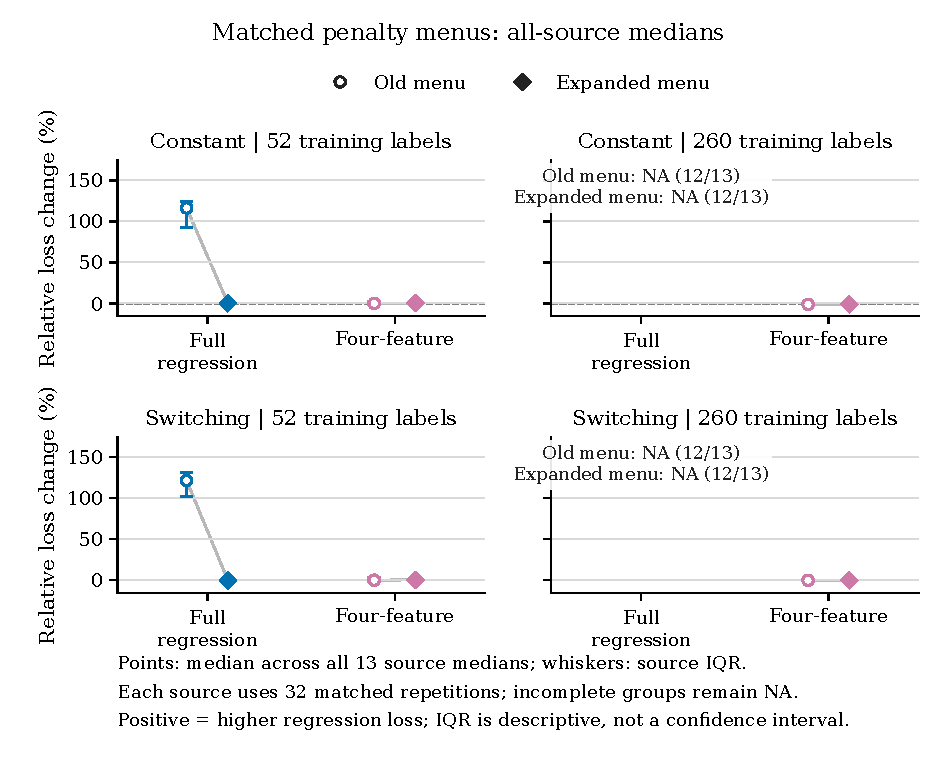
\includegraphics[width=.98\linewidth]{figures/v10-menu-isolation.pdf}
\caption{Paired penalty-menu isolation on unchanged calibrated paths. The expanded menu removes the large short-history full-regression loss in both arms. Longer-history full-regression summaries remain unavailable because a required repetition fails in each arm, with no successful-subset replacement.}\label{fig:mechanism}
\end{figure}

\FloatBarrier

\section{FX aggregation and additional forecast comparisons}\label{sup:levy-empirical}\label{sup:wp2-pairs}\label{sup:wp4}\label{sup:v8-daily}\label{sup:v8-backcast}

The pinned hourly FX snapshot produces 930 nonempty source-naive calendar
days under the fixed last-observation rule, rather than the approximate sample
size in the planning instruction. Each report is issued only at the end of its
completed source-naive day; the selected row's original timestamp is not treated
as an earlier time at which the identity of the last row was already known.
Missing days stay absent, and partial boundary days remain. The timezone and
historical first-release availability are unknown. This is a last-record proxy,
not a verified financial close or a peak over intraday excursions.

Histories and horizons count subsequent nonempty daily observations. The split
copies the Treasury observation-index geometry, not its absolute calendar dates
or a proportional split: validation runs from 2015-02-24 to 2015-04-24 and evaluation from
2015-05-24 to 2016-12-27 on 501 common issues. Raw or resampled positions
and per-issue trajectories are not redistributed.

Table~\ref{tab:daily-fx} reports every same-dealer daily comparison.
\begingroup\small\setlength{\tabcolsep}{3pt}
\begin{longtable}{rrlrrrr}
\caption{Same-dealer daily sampled-position results; history and horizon count recorded nonempty calendar days. All methods share the declared evaluation grid; loss is scaled to USD millions for display only. The four-feature report yielding the isolated score gain has more breaches than its historical reference.}\label{tab:daily-fx}\\
\toprule
History & Horizon & Procedure & Penalty & \shortstack{Mean loss\\(USD m)} & \shortstack{Loss change\\vs historical (\%)} & \shortstack{Breaches\\count / rate (\%)}\\\midrule
\endfirsthead
\caption[]{Continued.}\\\toprule
History & Horizon & Procedure & Penalty & \shortstack{Mean loss\\(USD m)} & \shortstack{Loss change\\vs historical (\%)} & \shortstack{Breaches\\count / rate (\%)}\\\midrule
\endhead
\bottomrule\endfoot
52 & 6 & Historical headroom & -- & 1.049 & -- & 36 / 7.186\\
52 & 6 & 33-feature regression & 0.1 & 2.032 & 93.586 & 146 / 29.142\\
52 & 6 & Four-feature regression & 0.001 & 1.974 & 88.128 & 129 / 25.749\\
52 & 24 & Historical headroom & -- & 1.553 & -- & 66 / 13.174\\
52 & 24 & 33-feature regression & 0.01 & 3.456 & 122.589 & 206 / 41.118\\
52 & 24 & Four-feature regression & 0.01 & 3.163 & 103.719 & 225 / 44.910\\
260 & 6 & Historical headroom & -- & 0.964 & -- & 30 / 5.988\\
260 & 6 & 33-feature regression & 0.1 & 1.175 & 21.873 & 54 / 10.778\\
260 & 6 & Four-feature regression & 0.1 & 0.935 & -2.974 & 37 / 7.385\\
260 & 24 & Historical headroom & -- & 1.882 & -- & 24 / 4.790\\
260 & 24 & 33-feature regression & 0.001 & 2.642 & 40.335 & 99 / 19.760\\
260 & 24 & Four-feature regression & 0.001 & 2.177 & 15.627 & 46 / 9.182\\
\end{longtable}
\endgroup


Historical headroom wins seven of the eight named comparisons, but the
four-feature longer-history, shorter-horizon daily exception lowers loss by
about 3.0\% with 37 regression breaches versus 30 historical breaches.
Both regressions meet the fixed majority-based descriptive classification,
not a dominance or coverage theorem. The recorded source identity is held fixed while physical history, horizon, update cadence, calendar predictors, sampled response and evaluation span change jointly. The contrast cannot
identify a pure frequency effect or supply independent dealer validation.

The endpoint plug-in uses each completed historical episode's
absolute endpoint displacement and adds its specified empirical quantile to
the actual current-position floor. It shares the historical rule's completed
origin pool and fixed refit schedule, with no fitted tuning parameter.
The operational empirical rank and overlapping financial history are distinct
from the known population quantile in the classical proposition. The report
therefore has to earn its financial coverage and score performance empirically.
The original tables in the extended results report every endpoint plug-in comparison and the separate working-reference contrasts.

The states are low, middle and high issue-known RMS position-change
states, not price volatility or yield regimes. Cutpoints come only from the
training history. Reports and original primary means stay unchanged; the
diagnostic divides the already viewed evaluation record without estimating a
switching policy. Source-native group differences are not pooled.

Comparing wrapped regression with wrapped historical reports is a
different question from comparing either wrapper with its unwrapped base.
The \href{https://github.com/ByronLi0207/financial-mathematics-paper-20261020/blob/submission-final/EXTENDED_RESULTS.md#asmbi-extended-s17}{extended calibration results} retain every within-cell comparison. A lower coverage distance measures closeness of the empirical hit rate to the target probability, not conditional coverage or lower monetary loss.

The fixed-prefix comparison overlaps the earlier inspected period. \href{https://github.com/ByronLi0207/financial-mathematics-paper-20261020/blob/submission-final/EXTENDED_RESULTS.md#asmbi-extended-s26}{Every full-prefix and overlapping-window result} remains available; these records are not an independent financial holdout.

\FloatBarrier


\section{Weekly historical rules retain their adverse comparisons}\label{sup:panel}\label{sup:panel-second}\label{sup:panel-levy}\label{sup:selection}\label{sup:selection-failures}

Each cell compares the same peak target, completed past outcomes,
origin sequence, fixed refit schedule and native monetary units. The original
full regression, smaller predictor regression, expanded-ridge full regression
and ordinary empirical report all remain visible. The additional series are
related weekly aggregates, not independent individual-dealer replications.
Changes in predictors and changes in the ridge menu are distinct interventions.
Every listed comparison is post-result / exploratory.

The historical column gives mean pinball loss and strict hits. Other columns
give the saved percentage loss difference against that same historical rule and
strict hits; negative percentages favor the column method. Original full
regression, four-feature regression and expanded-menu full regression are
distinct fitted procedures.
I is the ordinary
empirical-quantile report, with the endpoint qualification in Section~\ref{sup:rank}.
Across the saved panel, expanded full-regression median excess
loss is 9.22 percent,
compared with 92.63 percent for the original menu. Expanded regression still loses in 34 cells.
This improvement does not erase the remaining failures or identify a causal
feature effect.

The earlier-period experiment applies the saved fixed selection rules
to familiar historical data. These origins already have validation and
evaluation roles in the current records, including actual rolling-fold
scoring. They cannot now be treated as untouched evidence for the expanded
backcast. The experiment remains retrospective, not external or prospective
validation. R0 denotes the fixed minimum-validation-loss rule. R2 is the predesignated main one-standard-error selection rule,
not a result-dependent replacement chosen for its subsequent performance.
The rule design precedes its calculations but follows earlier research results.

R1 adds the ordinary empirical quantile to the finite regression candidates.
R2 compares each candidate's validation losses with the same best-mean
candidate, using the paired-difference Bartlett-HAC standard error. Candidates
within that tolerance qualify, and the fixed rule prefers the strongest
shrinkage, including the empirical report. This paired HAC tolerance is a
time-series adaptation of a one-standard-error preference, not the textbook
formula, a significance test or a noninferiority guarantee. It does not account
for the whole uncertainty from selecting the best candidate on that segment.

R3 applies the same preference to prespecified earlier rolling folds and the
outer validation segment, with origin-equal weighting and maturity gaps.
Its HAC pairs use actual source-index distances rather than compressing gaps.
Without an eligible earlier fold, the saved design makes it identical to R2;
this is not a numerical fallback. Earlier-period results were sealed before
the already-inspected-period calculations that could reuse those origins.

Required validation-candidate failure blocks the dependent rule;
it is neither retried nor replaced by a shorter mean. The \href{https://github.com/ByronLi0207/financial-mathematics-paper-20261020/blob/submission-final/EXTENDED_RESULTS.md#asmbi-extended-s15}{extended selection results} list every incomplete report. Every listed row has the saved reason
\texttt{REQUIRED\_VALIDATION\_CANDIDATE\_FAILED}. Those failures remain part of
the evidence even though other rules in the same task can complete.

The expanded penalty menu reduces the earlier full-regression losses but does not satisfy all written improvement conditions. The earlier conservative selection also fails its protection, gain-retention and median-improvement conditions. \href{https://github.com/ByronLi0207/financial-mathematics-paper-20261020/blob/submission-final/EXTENDED_RESULTS.md#asmbi-extended-s11}{The first half} and \href{https://github.com/ByronLi0207/financial-mathematics-paper-20261020/blob/submission-final/EXTENDED_RESULTS.md#asmbi-extended-s12}{second half of the complete weekly panel}, \href{https://github.com/ByronLi0207/financial-mathematics-paper-20261020/blob/submission-final/EXTENDED_RESULTS.md#asmbi-extended-s13}{every endpoint-plug-in comparison}, and \href{https://github.com/ByronLi0207/financial-mathematics-paper-20261020/blob/submission-final/EXTENDED_RESULTS.md#asmbi-extended-s14}{all earlier selection outcomes} retain the adverse rows and unchanged denominators.

\FloatBarrier


\section{History-length predictions have partial support}\label{sup:v11-history}\label{sup:submission-wp2}

The earlier confirmation exercise applies its fixed pooled criteria to heavy-tailed, regime-switching and compound-Poisson innovation laws. Table~\ref{tab:v11-confirmation} reports every prewritten criterion, including the failed universal ordering prediction. Its history regions use method-specific thresholds estimated in the earlier source study; they are not an oracle rule for the financial data.

\begin{table}[htbp]\centering\small
\caption{Saved confirmation criteria for excess loss relative to matched historical headroom under additional synthetic innovation laws. Counts use the original fixed pooled denominators, including all counterexamples.}\label{tab:v11-confirmation}
\begin{tabular}{p{7.2cm}rrrr}\toprule
Prewritten criterion & Successes & Missing & Required & Result \\ \midrule
Positive excess loss in the low-history region & 47/48 & 0 & 80\% & Supported \\
Negative excess loss in the high-history region & 21/24 & 0 & 60\% & Supported \\
Four-feature loss never exceeds full-regression loss & 42/48 & 0 & 100\% & Not supported \\
\bottomrule\end{tabular}
\par\smallskip\begin{minipage}{.98\linewidth}\footnotesize
History regions use the method-specific thresholds fixed in the linked original design, conditional on the earlier threshold exercise; the history index excludes predictor dimension.
Full and four-feature regressions retain different original penalty menus, so their ordering does not isolate predictor dimension.
The universal ordering prediction is not supported; the complete records retain all counterexamples and candidate failures.
\end{minipage}\end{table}


The \href{https://github.com/ByronLi0207/financial-mathematics-paper-20261020/tree/revision-v11/evidence/v11/pr5-v9}{unchanged source records} retain the complete synthetic results, counterexamples and candidate failures. The \href{https://github.com/ByronLi0207/financial-mathematics-paper-20261020/blob/revision-v11/evidence/v11/pr5-v9/protocol/revision-v9/wp2-confirmatory.md}{original confirmation design} records the fixed laws, history regions, penalty menus and decision rules. The local design commits precede their numerical runs; the later public file uploads are not public preregistration.

The complete \href{https://github.com/ByronLi0207/financial-mathematics-paper-20261020/blob/revision-v11/evidence/v11/pr5-v9/results/revision-v9/wp3/contrasts.json}{FX history contrasts} retain both horizons and every tested window. Both longer-horizon methods lose their gain again at the longest history. The four-feature short-horizon first cutpoint is left-censored and not testable, so the original confirmation across all curves is not established. These comparisons use the inspected period and provide neither evidence from an additional dealer nor a fresh financial holdout.

This section imports saved results from the separately developed final-jof branch. The local design commit precedes calculation; public upload occurred after calculation. This is not an externally registered or prospective financial confirmation.

The shorter-history outcomes had already been inspected. Only the longest-history forecasts were added under the fixed extension design. The same downloaded CFTC source arrays and reporting-vintage limitations apply.

\begin{table}[htbp]\centering\small

\caption{Fixed history-length decision screens, including failed and untestable predictions. Counts use the original planned denominators.}\label{tab:submission-wp2}

\begin{tabular}{lllll}\toprule

Screen & Regression & Successes / planned & Required fraction & Judgment\\\midrule

P1 & Four-feature & 15 / 17 & 80\% & Supported\\

P1 & Full & 29 / 34 & 80\% & Supported\\

P2 & Four-feature & 10 / 17 & 60\% & Not supported\\

P2 & Full & --- & --- & Not testable\\

P3 & Four-feature & 6 / 17 & 70\% & Not supported\\

\bottomrule\end{tabular}\end{table}

Both low-history disadvantage screens pass. The longer-history advantage screen and strict sequential-improvement screen fail. The full regression has no prewritten high-region cell. The retained overall judgment is partial support.

\href{https://github.com/ByronLi0207/financial-mathematics-paper-20261020/blob/submission-final/EXTENDED_RESULTS.md#asmbi-extended-s39}{Every saved CFTC counterexample, with its original signed loss change}, remains alongside the complete source rows. Markets can appear under several screens; ties remain failures of strict ordering.

\FloatBarrier


\section{Historical methods remain in most confidence sets}\label{sup:v10-mcs}\label{sup:v13-mcs}

Joint comparison leaves matched historical methods alongside alternatives in most sets, with a single historical method surviving in only a small minority. These results support retaining historical controls while leaving many alternatives uneliminated under the fixed bootstrap approximation. Non-elimination does not establish equal predictive risk. Table~\ref{tab:v10-mcs-main} reports surviving methods, with identical observed-loss patterns explained separately in \href{https://github.com/ByronLi0207/financial-mathematics-paper-20261020/blob/submission-final/EXTENDED_RESULTS.md#asmbi-extended-s31}{the complete confidence-set archive}. \href{https://github.com/ByronLi0207/financial-mathematics-paper-20261020/blob/submission-final/EXTENDED_RESULTS.md#asmbi-extended-s31}{The complete confidence-set archive} retains every set, method p-value, equivalence class and prior unavailable method.

These confidence sets use the original comparison inventory; the later validation rules are reported separately in Section~\ref{sup:v13-checks}.

\begin{table}[!htbp]\centering\footnotesize
\setlength{\tabcolsep}{4pt}
\caption{Ninety-percent model confidence sets across all planned comparisons. Counts retain their comparison or conditional-procedure denominators.}\label{tab:v10-mcs-main}
\begin{tabular}{lrrrrr}\toprule
Group & Complete & Matched history & Sole historical & Conditional & Unavailable \\
 & / planned & included & method & excluded & procedures \\ \midrule
FX original & 4/4 & \makebox[3.2em][r]{2/4} (\makebox[2.9em][r]{50.0}\%) & \makebox[3.2em][r]{0/4} (\makebox[2.9em][r]{0.0}\%) & \makebox[3.2em][r]{39/66} (\makebox[2.9em][r]{59.1}\%) & 6 \\
FX earlier period & 4/4 & \makebox[3.2em][r]{3/4} (\makebox[2.9em][r]{75.0}\%) & \makebox[3.2em][r]{0/4} (\makebox[2.9em][r]{0.0}\%) & \makebox[3.2em][r]{1/15} (\makebox[2.9em][r]{6.7}\%) & 2 \\
Treasury bills & 4/4 & \makebox[3.2em][r]{4/4} (\makebox[2.9em][r]{100.0}\%) & \makebox[3.2em][r]{0/4} (\makebox[2.9em][r]{0.0}\%) & \makebox[3.2em][r]{11/74} (\makebox[2.9em][r]{14.9}\%) & 4 \\
Other NYFed panels & 48/48 & \makebox[3.2em][r]{46/48} (\makebox[2.9em][r]{95.8}\%) & \makebox[3.2em][r]{0/48} (\makebox[2.9em][r]{0.0}\%) & \makebox[3.2em][r]{110/384} (\makebox[2.9em][r]{28.6}\%) & 48 \\
Same-record daily FX & 4/4 & \makebox[3.2em][r]{4/4} (\makebox[2.9em][r]{100.0}\%) & \makebox[3.2em][r]{2/4} (\makebox[2.9em][r]{50.0}\%) & \makebox[3.2em][r]{5/8} (\makebox[2.9em][r]{62.5}\%) & 0 \\
CFTC & 34/34 & \makebox[3.2em][r]{31/34} (\makebox[2.9em][r]{91.2}\%) & \makebox[3.2em][r]{0/34} (\makebox[2.9em][r]{0.0}\%) & \makebox[3.2em][r]{31/136} (\makebox[2.9em][r]{22.8}\%) & 0 \\
All comparisons & 98/98 & \makebox[3.2em][r]{90/98} (\makebox[2.9em][r]{91.8}\%) & \makebox[3.2em][r]{2/98} (\makebox[2.9em][r]{2.0}\%) & \makebox[3.2em][r]{197/683} (\makebox[2.9em][r]{28.8}\%) & 60 \\
\bottomrule\end{tabular}
\par\smallskip\begin{minipage}{.98\linewidth}\footnotesize
Matched history includes corrected and ordinary empirical headroom reports, excluding rolling references and nearest-neighbor baselines; conditional exclusions count complete procedures.
Identical losses can leave several methods tied, so the sole-method column counts only sets containing exactly one historical procedure.
\href{https://github.com/ByronLi0207/financial-mathematics-paper-20261020/blob/submission-final/EXTENDED_RESULTS.md#asmbi-extended-s31}{The complete confidence-set archive} retains all tied loss patterns, secondary membership counts and unavailable procedures; related comparisons are not independent replications.
\end{minipage}\end{table}

\FloatBarrier


\section{Scores, breaches and specified limit costs}\label{sup:preference}\label{sup:frontier-0}\label{sup:wp3-murphy}\label{sup:v10-cost}\label{sup:v10-diagnostics}

For a fixed report, changing the loss weight traces a line
\(R_a=aU+(1-a)V\). Here, \(U=\operatorname{mean}(P-C)_+\) is mean underprediction and
\(V=\operatorname{mean}(C-P)_+\) is mean overprediction. These are passive error amounts over all
origins, not observed funding costs. Breach frequency averages an indicator and
need not rank reports like either amount. These source-reported monetary values are never pooled across FX and weekly aggregates.

For each comparison, let $B$ be the issue-known floor, $Y$ the realized sampled peak,
$C_m$ a saved method report, and $m_F=\overline{C_F-B}>0$ the matched F report's
mean reserved headroom. All four quantities use the same source-native position
units (currency or contract counts). The normalized per-issue cost is
\[
J_m(\kappa,\beta,c)=\kappa\frac{\overline{C_m-B}}{m_F}
+\beta\,\overline{\mathbf 1\{Y>C_m\}}
+c\frac{\overline{(Y-C_m)_+}}{m_F},\qquad b=\beta m_F.
\]
Reserve, strict breach frequency and excess enter separately. The fixed breach
charge $b$ is in those same position-value units; each $\beta$ scales it to that
comparison's evaluation-sample F headroom. Charges therefore differ across
comparisons. Costs apply per issued report; overlapping horizons are not
added as separate cash flows.
The fixed grid is $\kappa\in\{.01,.025,.05,.1,.2,.5,1\}$,
$\beta\in\{0,.01,.05,.1,.25,.5,1,2,5\}$ and $c\in\{.5,1,2\}$.
At $\kappa=.05,\beta=0,c=1$, the cost difference from F is the pinball-loss
difference divided by $m_F$. Other weights need not preserve that ranking.
The panels compare fixed reports and do not estimate a cost-optimal policy.

All 98 comparisons have a positive scale and all 976 complete methods enter 189 grid points, giving 184,464 cost rows. Sixteen missing-floor inputs are recovered only from their pre-specified, fingerprinted same-origin F copies. Their complete origin, target and floor arrays match exactly. Other missing or mismatched floors would make the whole comparison unavailable. No missing scale uses an epsilon.

The public \texttt{results/v10/cost/cost-grid.csv.zip} contains every complete method's normalized mean cost, its F reference and strict cheaper/equal status at all coefficients. \texttt{primary-regions.csv} retains all 18,522 planned primary grid rows, including status fields. Primitive reserve amounts, strict breach counts/rates and excess amounts appear in \texttt{primitive-stats.json}. Source-group figures use the full planned comparison denominators. The primary comparison is fixed expanded-menu full regression for hourly/weekly/CFTC sources and the original saved regression for daily FX. Other methods retain separate regions and are never replaced by a minimum-cost oracle.

\href{https://github.com/ByronLi0207/financial-mathematics-paper-20261020/blob/submission-final/EXTENDED_RESULTS.md#asmbi-extended-s09}{All original fixed-report error amounts and weight crossings} and \href{https://github.com/ByronLi0207/financial-mathematics-paper-20261020/blob/submission-final/EXTENDED_RESULTS.md#asmbi-extended-s19}{all combination-score crossings} retain the complete comparisons.

\begin{figure}[htbp]\centering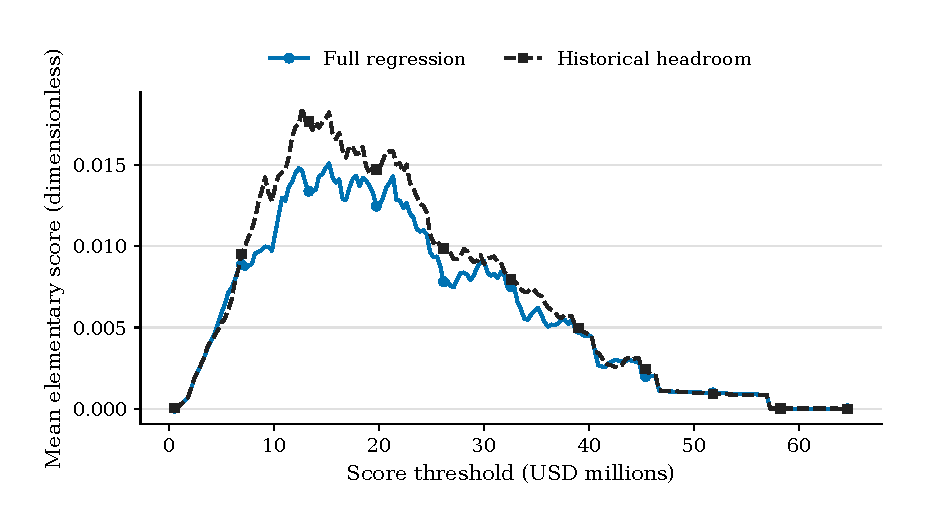
\includegraphics[width=.94\linewidth]{figures/v7-murphy-fx_hourly.pdf}
\caption{Murphy diagram for the main short-horizon FX comparison. The full-breakpoint calculation finds crossings; the graph is a display of saved scores. Average pinball superiority does not imply dominance across elementary scores.}\label{fig:murphyfx}
\end{figure}\begin{figure}[htbp]\centering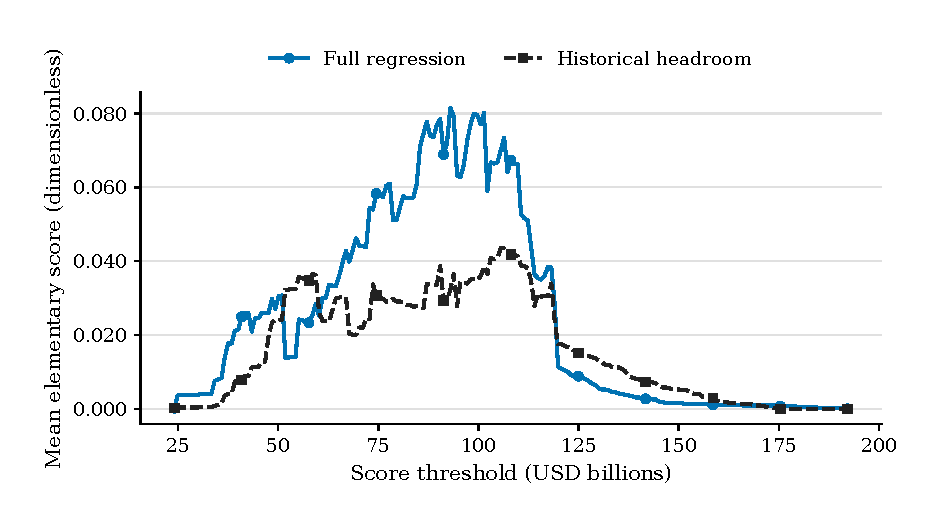
\includegraphics[width=.94\linewidth]{figures/v7-murphy-nyfed_weekly.pdf}
\caption{Murphy diagram for the main Treasury-bill comparison. The saved full-breakpoint comparison also crosses. A single average-score ordering leaves other consistent-score preferences unresolved.}\label{fig:murphybill}
\end{figure}



\FloatBarrier


\section{Longer validation improves medians but leaves losses}\label{sup:v13-checks}

\paragraph{Longer validation in the New York Fed series.}
Across-series median loss falls under longer validation at both horizons, extending the direction found in CFTC. Main Table 7 reports full regression. \href{https://github.com/ByronLi0207/financial-mathematics-paper-20261020/blob/submission-final/EXTENDED_RESULTS.md#asmbi-extended-s38}{The complete validation results} retain the four-feature variant, its failed short-horizon median-improvement condition, and every source-by-source sequence without pooling their evidence.

The complete validation summary is in Main Table 7.


The original validation origins are 329--380; longer validation uses 243--398 at the short horizon and 225--380 at the longer horizon. Evaluation remains 405--681, with 277 issues. Thus the short-horizon endpoint also advances eighteen weeks and changes the validation refit phase; this is not a causal length-only comparison. The longer-horizon endpoint is unchanged. Differences between medians for each design also need not describe a typical series: for full regression, the paired-change median is +0.00 and -44.10 percentage points, respectively. All source, candidate and failure records remain in the \href{https://github.com/ByronLi0207/financial-mathematics-paper-20261020/tree/revision-v13/results/v13/nyfed-validation}{complete validation-length results}; related weekly categories are not independent dealer replications.

The unchanged source-by-source validation plot is retained in \href{https://github.com/ByronLi0207/financial-mathematics-paper-20261020/blob/submission-final/EXTENDED_RESULTS.md#asmbi-extended-s38}{validation records}.


\FloatBarrier
\paragraph{The retrospective validation protocol.}
The rule uses the six-point penalty menu, longer validation, and a historical default. Weekly validation contains 156 issues and FX validation contains 5,760; regression replaces corrected historical headroom only when its validation advantage exceeds one paired HAC standard error. Selection and the gate share validation data, and the decision stays fixed over the evaluation segment. Infinite shrinkage gives ordinary empirical headroom, so it must pass the same gate to replace the corrected-rank reference. These settings combine existing forecasting and validation methods without a nominal protection guarantee.

All 62 planned comparisons complete, including 60 weekly cells and both FX periods. The weekly median moves from +14.63\% for ordinary regression with the six-point menu to 0.00\% for the protocol. However, 8 of 60 weekly cells exceed the historical loss by more than 10\%, and the worst excess is +80.98\%. The median condition therefore passes while the tail condition fails. The protocol returns to history in 32 weekly cells and uses regression in 28, as Table~\ref{tab:v13-routing} shows. The adverse cells comprise 7 CFTC comparisons and 1 New York Fed comparison. Both FX periods retain their ordinary-regression gains, 14.77\% and 16.62\%, meeting the gain-retention condition.

\begin{table}[!htbp]\centering\footnotesize\setlength{\tabcolsep}{4pt}
\caption{Historical selections and adverse outcomes by source, horizon and training history. Counts use every planned comparison in each row; the last column counts protocol excess loss above ten percent.}\label{tab:v13-routing}
\begin{tabular}{lrrr rr}\toprule
Source / period & $H$ & $W$ & Historical choice & Median excess (\%) & Adverse count\\\midrule
Treasury bills & 6 & 52 & 1 / 1 & +0.00 & 0 \\
Other NY Fed series & 6 & 52 & 8 / 12 & +0.00 & 1 \\
Treasury bills & 24 & 52 & 1 / 1 & +0.00 & 0 \\
Other NY Fed series & 24 & 52 & 10 / 12 & +0.00 & 0 \\
CFTC & 6 & 52 & 6 / 17 & +0.00 & 4 \\
CFTC & 6 & 260 & 6 / 17 & +0.00 & 3 \\
FX, original & 6 & 2880 & 0 / 1 & -14.77 & 0 \\
FX, earlier & 6 & 2880 & 0 / 1 & -16.62 & 0 \\
\bottomrule\end{tabular}
\end{table}

The adverse CFTC cells are 1170E1, 095741, 232741 and 112741 at the shorter history, and 044601, 096742 and 112741 at the longer history. The remaining cell is the New York Fed two-to-three-year Treasury coupon category at the short horizon. The \href{https://github.com/ByronLi0207/financial-mathematics-paper-20261020/tree/revision-v13/results/v13/recommended-protocol}{complete protocol results} retain every comparison, selected penalty, paired gate and fallback route. The protocol was designed after inspecting earlier results, including these evaluation periods, so this is a retrospective test rather than prospective protection evidence.

\FloatBarrier


\section{Numerical rejection and retrospective timing}\label{sup:wp5}\label{sup:reproduction}\label{sup:v12-details}

At the 99\% quantile, required numerical fits fail in one CFTC comparison and both FX periods. A post-failure solver repair reproduces forecasts within $10^{-6}$ pointwise relative error in only 6 of 10 previously converged fits. Unchanged residual and duality-gap thresholds reject this repair, preventing all three failed comparisons from running with the change. Their original unavailable values and both undetermined tail-level judgments remain in the \href{https://github.com/ByronLi0207/financial-mathematics-paper-20261020/tree/revision-v13/results/v13/tau-repair}{complete numerical check}, including every compatibility failure and unrun comparison.

The original FX evaluation period was inspected before the conditional extension. Later written designs retain their own local-commit and public-upload chronology; public posting after calculation is not public preregistration. Complete audit and execution records remain in \href{https://github.com/ByronLi0207/financial-mathematics-paper-20261020/blob/submission-final/EXTENDED_RESULTS.md#asmbi-extended-s36}{earlier scope records}, \href{https://github.com/ByronLi0207/financial-mathematics-paper-20261020/blob/submission-final/EXTENDED_RESULTS.md#asmbi-extended-s38}{validation records}, and \href{https://github.com/ByronLi0207/financial-mathematics-paper-20261020/blob/submission-final/EXTENDED_RESULTS.md#asmbi-extended-s39}{history-extension records}.

The repository provides the code, protocols, saved aggregate results and source acquisition instructions. Financial replay still requires the documented compatible raw inputs and historical code; public summaries alone do not supply those inputs.

\FloatBarrier


\section{Written predictions and saved judgments}\label{sup:submission-predictions}

These decisions are copied from the saved register, including every unsupported and undetermined screen. Written-before-run status is distinct from external preregistration and prospective financial evaluation. The full threshold, numerical output, original status, timing record and source pointer for every row remain in \href{https://github.com/ByronLi0207/financial-mathematics-paper-20261020/blob/submission-final/EXTENDED_RESULTS.md#asmbi-extended-s40}{the complete six-column register}.

{\footnotesize
\begin{longtable}{p{2.0cm}p{10.5cm}p{2.5cm}}
\caption{Every saved written prediction and decision. Full numerical outputs, exact status reasons and source bindings remain in the extended results.}\label{tab:submission-predictions}\\
\toprule Screen & Written criterion & Saved judgment\\\midrule\endfirsthead
\toprule Screen & Written criterion & Saved judgment\\\midrule\endhead
\texttt{E5.\allowbreak{}P1.\allowbreak{}QR33\ensuremath{+}} & QR33+ strictly improves original QR33 loss within the 45 originally adverse panel cells.\par\emph{Threshold:} At least 40 of fixed 45 cells. & Not supported \\[3pt]
\texttt{E5.\allowbreak{}P2.\allowbreak{}QR33\ensuremath{+}} & QR33+ excess loss against F lies within inclusive [-10\%,\allowbreak{} +10\%].\par\emph{Threshold:} At least 36 of fixed 48 cells within [-10,\allowbreak{} +10]\%. & Not supported \\[3pt]
\texttt{E5.\allowbreak{}P3.\allowbreak{}QR33\ensuremath{+}} & Selected ridge penalty is at least 1.\par\emph{Threshold:} At least 25 of fixed 48 cells (more than half). & Supported \\[3pt]
\texttt{R6.\allowbreak{}S1.\allowbreak{}R2} & All 26 retrospective weekly R2 cells complete with bounded worst and median excess.\par\emph{Threshold:} 26/\allowbreak{}26 complete; worst \ensuremath{<}=\allowbreak{} +25\%; median \ensuremath{<}=\allowbreak{} +5\%. & Not supported \\[3pt]
\texttt{R6.\allowbreak{}S2.\allowbreak{}R2} & R2 retains at least half of each negative R0 FX H6 gain.\par\emph{Threshold:} For each eligible R0 \ensuremath{<} 0 cell,\allowbreak{} R2 \ensuremath{<}=\allowbreak{} 0.5*R0; at least one eligible cell required. & Not supported \\[3pt]
\texttt{R6.\allowbreak{}S3.\allowbreak{}R2} & R2 weekly median excess is strictly lower than R0.\par\emph{Threshold:} Both rules complete 26 cells; median(R2) \ensuremath{<} median(R0). & Not supported \\[3pt]
\texttt{E1.\allowbreak{}M1.\allowbreak{}QR33} & At W52, the QR33 median with constant parameters is near parity with F.\par\emph{Threshold:} Inclusive [-5,\allowbreak{} +5]\%. & Supported \\[3pt]
\texttt{E1.\allowbreak{}M2.\allowbreak{}QR33} & At W52, the QR33 median with switching parameters exceeds the constant-parameter median by 5 pp.\par\emph{Threshold:} Switching minus constant \ensuremath{>}=\allowbreak{} +5 pp. & Not supported \\[3pt]
\texttt{E1.\allowbreak{}M3.\allowbreak{}QR33} & Both group medians improve and at least 12 of 13 sources improve in both groups.\par\emph{Threshold:} Both group medians strictly lower; joint improvement \ensuremath{>}=\allowbreak{} 12/\allowbreak{}13. & Supported \\[3pt]
\texttt{E2.\allowbreak{}T1.\allowbreak{}QR33} & Realized better historical report min(F,\allowbreak{} I) strictly beats QR33.\par\emph{Threshold:} At least 60\% of all 2K cells; no missing operand deletion. & Supported \\[3pt]
\texttt{E2.\allowbreak{}T2.\allowbreak{}QR33} & Each W QR33 median excess against F lies near parity.\par\emph{Threshold:} Inclusive [-10,\allowbreak{} +10]\% at both W52 and W260. & Not supported \\[3pt]
\texttt{E2.\allowbreak{}T3.\allowbreak{}QR4} & QR4 median excess is strictly lower with W260 than W52.\par\emph{Threshold:} W260 median \ensuremath{<} W52 median. & Supported \\[3pt]
\texttt{F1.\allowbreak{}D1.\allowbreak{}QR33} & Strictly positive finite-menu oracle gap G in more than half of fixed 41 short-weekly cells.\par\emph{Threshold:} Fixed 41 denominator; positive G share \ensuremath{>} 1/\allowbreak{}2,\allowbreak{} using missing bounds. & Supported \\[3pt]
\texttt{F1.\allowbreak{}D2.\allowbreak{}QR33} & Positive actual excess E and selection component S \ensuremath{>} E/\allowbreak{}2 in more than half of fixed 41 cells.\par\emph{Threshold:} Fixed 41 denominator; share of E \ensuremath{>} 0 and S \ensuremath{>} E/\allowbreak{}2 \ensuremath{>} 1/\allowbreak{}2,\allowbreak{} using missing bounds. & Supported \\[3pt]
\texttt{F1.\allowbreak{}D3.\allowbreak{}QR33} & Both original long-history FX horizons have negative finite-menu gap.\par\emph{Threshold:} G \ensuremath{<} 0 at H6 and H24; conjunction of both original FX cells. & Supported \\[3pt]
\texttt{F2.\allowbreak{}V1.\allowbreak{}QR33} & At each W, longer CFTC validation reduces the across-contract QR33 median by at least 5 pp.\par\emph{Threshold:} For each W52/\allowbreak{}W260: median(V156)-median(V52) \ensuremath{<}=\allowbreak{} -5 pp; both required. & Supported \\[3pt]
\texttt{F2.\allowbreak{}V2.\allowbreak{}QR33} & Longer CFTC validation raises empirical-limit selection frequency at each W.\par\emph{Threshold:} At each W52/\allowbreak{}W260: infinity count(V156) \ensuremath{>} count(V52); both required. & Supported \\[3pt]
\texttt{F3.\allowbreak{}Q1.\allowbreak{}QR33} & At tau .99 F strictly beats QR33 in at least 29 fixed CFTC cells.\par\emph{Threshold:} At least 29/\allowbreak{}34; strict wins only; fixed denominator with unknown bounds. & Undetermined \\[3pt]
\texttt{F3.\allowbreak{}Q2.\allowbreak{}QR33} & At tau .99 QR33 improves matched F in both FX periods.\par\emph{Threshold:} Relative excess \ensuremath{<} 0 in original and early 2015; both required. & Undetermined \\[3pt]
\texttt{G2.\allowbreak{}V3.\allowbreak{}QR33} & At each horizon, longer New York Fed validation reduces the median across 13 series by at least 5 pp.\par\emph{Threshold:} At each H6/\allowbreak{}H24: median(V156)-median(V52) \ensuremath{<}=\allowbreak{} -5 pp; both required. & Supported \\[3pt]
\texttt{G2.\allowbreak{}V4.\allowbreak{}QR33} & Longer NY Fed validation increases empirical-limit selections at each horizon.\par\emph{Threshold:} At each H6/\allowbreak{}H24: infinity count(V156) \ensuremath{>} count(V52); both required. & Supported \\[3pt]
\texttt{G3.\allowbreak{}R1.\allowbreak{}RP} & Protocol median excess is small across all 60 eligible weekly cells.\par\emph{Threshold:} Full-universe median \ensuremath{<}=\allowbreak{} +1\%; any eligible missing outcome =\allowbreak{}\ensuremath{>} UNDETERMINED. & Supported \\[3pt]
\texttt{G3.\allowbreak{}R2.\allowbreak{}RP} & At most 5\% of eligible weekly cells lose more than 10\% against F.\par\emph{Threshold:} Adverse defined excess \ensuremath{>} 10\%; adverse fraction \ensuremath{<}=\allowbreak{} 0.05; at most 3 of 60. & Not supported \\[3pt]
\texttt{G3.\allowbreak{}R3.\allowbreak{}RP} & Retain at least half of ordinary QR gain in every eligible FX period.\par\emph{Threshold:} If ordinary excess \ensuremath{<} 0,\allowbreak{} RP excess \ensuremath{<}=\allowbreak{} 0.5*ordinary; every eligible gain period and at least 1 required. & Supported \\[3pt]
\texttt{WP2.\allowbreak{}P1\_QR4.\allowbreak{}QR4} & Low-region QR4 strictly loses against matched F.\par\emph{Threshold:} At least 80\% of fixed 17 low-region cells; combined P1 requires both methods. & Supported \\[3pt]
\texttt{WP2.\allowbreak{}P1\_QR33.\allowbreak{}QR33} & Low-region QR33 strictly loses against matched F.\par\emph{Threshold:} At least 80\% of fixed 34 low-region cells; combined P1 requires both methods. & Supported \\[3pt]
\texttt{WP2.\allowbreak{}P2\_QR4.\allowbreak{}QR4} & High-region W520 QR4 strictly beats matched F.\par\emph{Threshold:} At least 60\% of fixed 17 high-region cells. & Not supported \\[3pt]
\texttt{WP2.\allowbreak{}P2\_QR33.\allowbreak{}QR33} & QR33 high-region comparison requires observed c \ensuremath{>} 2 r*.\par\emph{Threshold:} No registered high-region cell exists; structurally NOT\_\allowbreak{}TESTABLE by design. & Undetermined \\[3pt]
\texttt{WP2.\allowbreak{}P3\_QR4.\allowbreak{}QR4} & QR4 excess loss strictly decreases at both successive history steps.\par\emph{Threshold:} At least 70\% of fixed 17 markets satisfy Delta 52 \ensuremath{>} Delta 260 \ensuremath{>} Delta 520. & Not supported \\[3pt]
\texttt{F1.\allowbreak{}D1.\allowbreak{}QR4} & Strictly positive finite-menu oracle gap G in more than half of fixed 41 short-weekly cells.\par\emph{Threshold:} Fixed 41 denominator; positive G share \ensuremath{>} 1/\allowbreak{}2,\allowbreak{} using missing bounds. & Supported \\[3pt]
\texttt{F1.\allowbreak{}D2.\allowbreak{}QR4} & Positive actual excess E and selection component S \ensuremath{>} E/\allowbreak{}2 in more than half of fixed 41 cells.\par\emph{Threshold:} Fixed 41 denominator; share of E \ensuremath{>} 0 and S \ensuremath{>} E/\allowbreak{}2 \ensuremath{>} 1/\allowbreak{}2,\allowbreak{} using missing bounds. & Supported \\[3pt]
\texttt{F1.\allowbreak{}D3.\allowbreak{}QR4} & Both original long-history FX horizons have negative finite-menu gap.\par\emph{Threshold:} G \ensuremath{<} 0 at H6 and H24; conjunction of both original FX cells. & Supported \\[3pt]
\texttt{F2.\allowbreak{}V1.\allowbreak{}QR4} & At each W, longer CFTC validation reduces the across-contract QR4 median by at least 5 pp.\par\emph{Threshold:} For each W52/\allowbreak{}W260: median(V156)-median(V52) \ensuremath{<}=\allowbreak{} -5 pp; both required. & Undetermined \\[3pt]
\texttt{F2.\allowbreak{}V2.\allowbreak{}QR4} & Longer CFTC validation raises empirical-limit selection frequency at each W.\par\emph{Threshold:} At each W52/\allowbreak{}W260: infinity count(V156) \ensuremath{>} count(V52); both required. & Undetermined \\[3pt]
\texttt{G2.\allowbreak{}V3.\allowbreak{}QR4} & At each horizon, longer New York Fed validation reduces the median across 13 series by at least 5 pp.\par\emph{Threshold:} At each H6/\allowbreak{}H24: median(V156)-median(V52) \ensuremath{<}=\allowbreak{} -5 pp; both required. & Not supported \\[3pt]
\texttt{G2.\allowbreak{}V4.\allowbreak{}QR4} & Longer NY Fed validation increases empirical-limit selections at each horizon.\par\emph{Threshold:} At each H6/\allowbreak{}H24: infinity count(V156) \ensuremath{>} count(V52); both required. & Supported \\[3pt]
\bottomrule\end{longtable}
}

\FloatBarrier

\end{document}
